\chapter{Vergleich}

Das folgende Kapitel die drei besprochenen Entscheidungssysteme vergleichen. Der Vergleich wird sich auf die Implementierung und Performance fokussieren.

\section{FSM}

Die FSM kann bei komplexen Videospielen un�bersichtlich werden. So hatte das Spiel Half-Life (1998) ca. 80 so genannte Tasks, welche alle einem Zustand zugewiesen sind. Die FSM ist schwer skalierbar. �ndert man Aktionen oder m�chte man neue Aktionen hinzuf�gen, so muss der Graph der FSM angepasst werden, indem Zust�nde ge�ndert oder neue hinzugef�gt werden. Diese Zust�nde sollen zu einer logischen Spielmechanik des NPC f�hren, die FSM soll Zust�nde korrekt w�hlen. Zust�nde und �berg�nge sollten dabei vollst�ndig definiert sein. �nderungen f�hren zu Zeitaufwand, da der NPC getestet werden muss. Au�erdem k�nnen Leistungsprobleme auftreten, insbesondere bei einer �berm��igen Anzahl von Zust�nden.\autocite{U2023}
Eine Finite State Machine (FSM) wird h�ufig f�r einfache NPC-Logiken empfohlen, da ihr Design, die Implementierung, Visualisierung und das Debuggen vergleichsweise einfach sind. Doch mit der gr��e des Spieles steigt der Aufwand die FSM umzusetzen, da sie viel zu unflexibel und undynamisch ist.\autocite{review_game_ai} Im Punkt der Skalierbarkeit ist sie GOAP unterlegen.\autocite{Schwab2021}


%So besitzt \textit{Half-Life (1998)} X Zust�nde, welche �ber eine HFSM �bersichtlicher w�ren.
%\autocite{U2023}

%Diese Einschr�nkungen f�hrten dazu, dass die Spieleindustrie nach alternativen Methoden f�r die Entscheidungsfindung von NPCs suchte. Ein Beispiel hierf�r ist GOAP von Jeff Orkin, welches einen neuen Ansatz durch einen Suchalgorithmus entwickelte.


%- With recent technological developments, FSMs, DTs and BTs for managing decisions of NPCs are deficient in some situations, such as bad performance on overgrown tree structures, repeating mistakes without learning, and selecting the same decisions without being adaptive to different conditions creating the need for more believable character management methods

\section{BT}
\autocite{review_game_ai}:
BTs are more flexible to design and easier to test due to the modular design concept, which promotes its successful application in games such asHalo 2 and Bioshock. 

\section{GOAP}

%GOAP
\autocite{Schwab2021}:
 - GOAP system in not ideal though. First of all, it is resource-heavy thus it is impossible to reliably implement full-scale system on mobile platform (as of 2018 at least). Additionally, it is really hard to predict possible queue of actions which makes it hard to debug and a challenge to assign satisfying costs to every action.
 - FSM is most definitely not a viable alternative to GOAP. As stated in 1, its maintenance in ever-changing game development environment is too much of a hassle with complicated AI behavior. It is however the perfect solution for small projects because of it simplicity.
- BT is not perfect solution for more complicated AIs though. Developers need to spend a lot of time to create appropriate conditional nodes and link them with correct behaviors.

\begin{figure}[h]
  \centering
  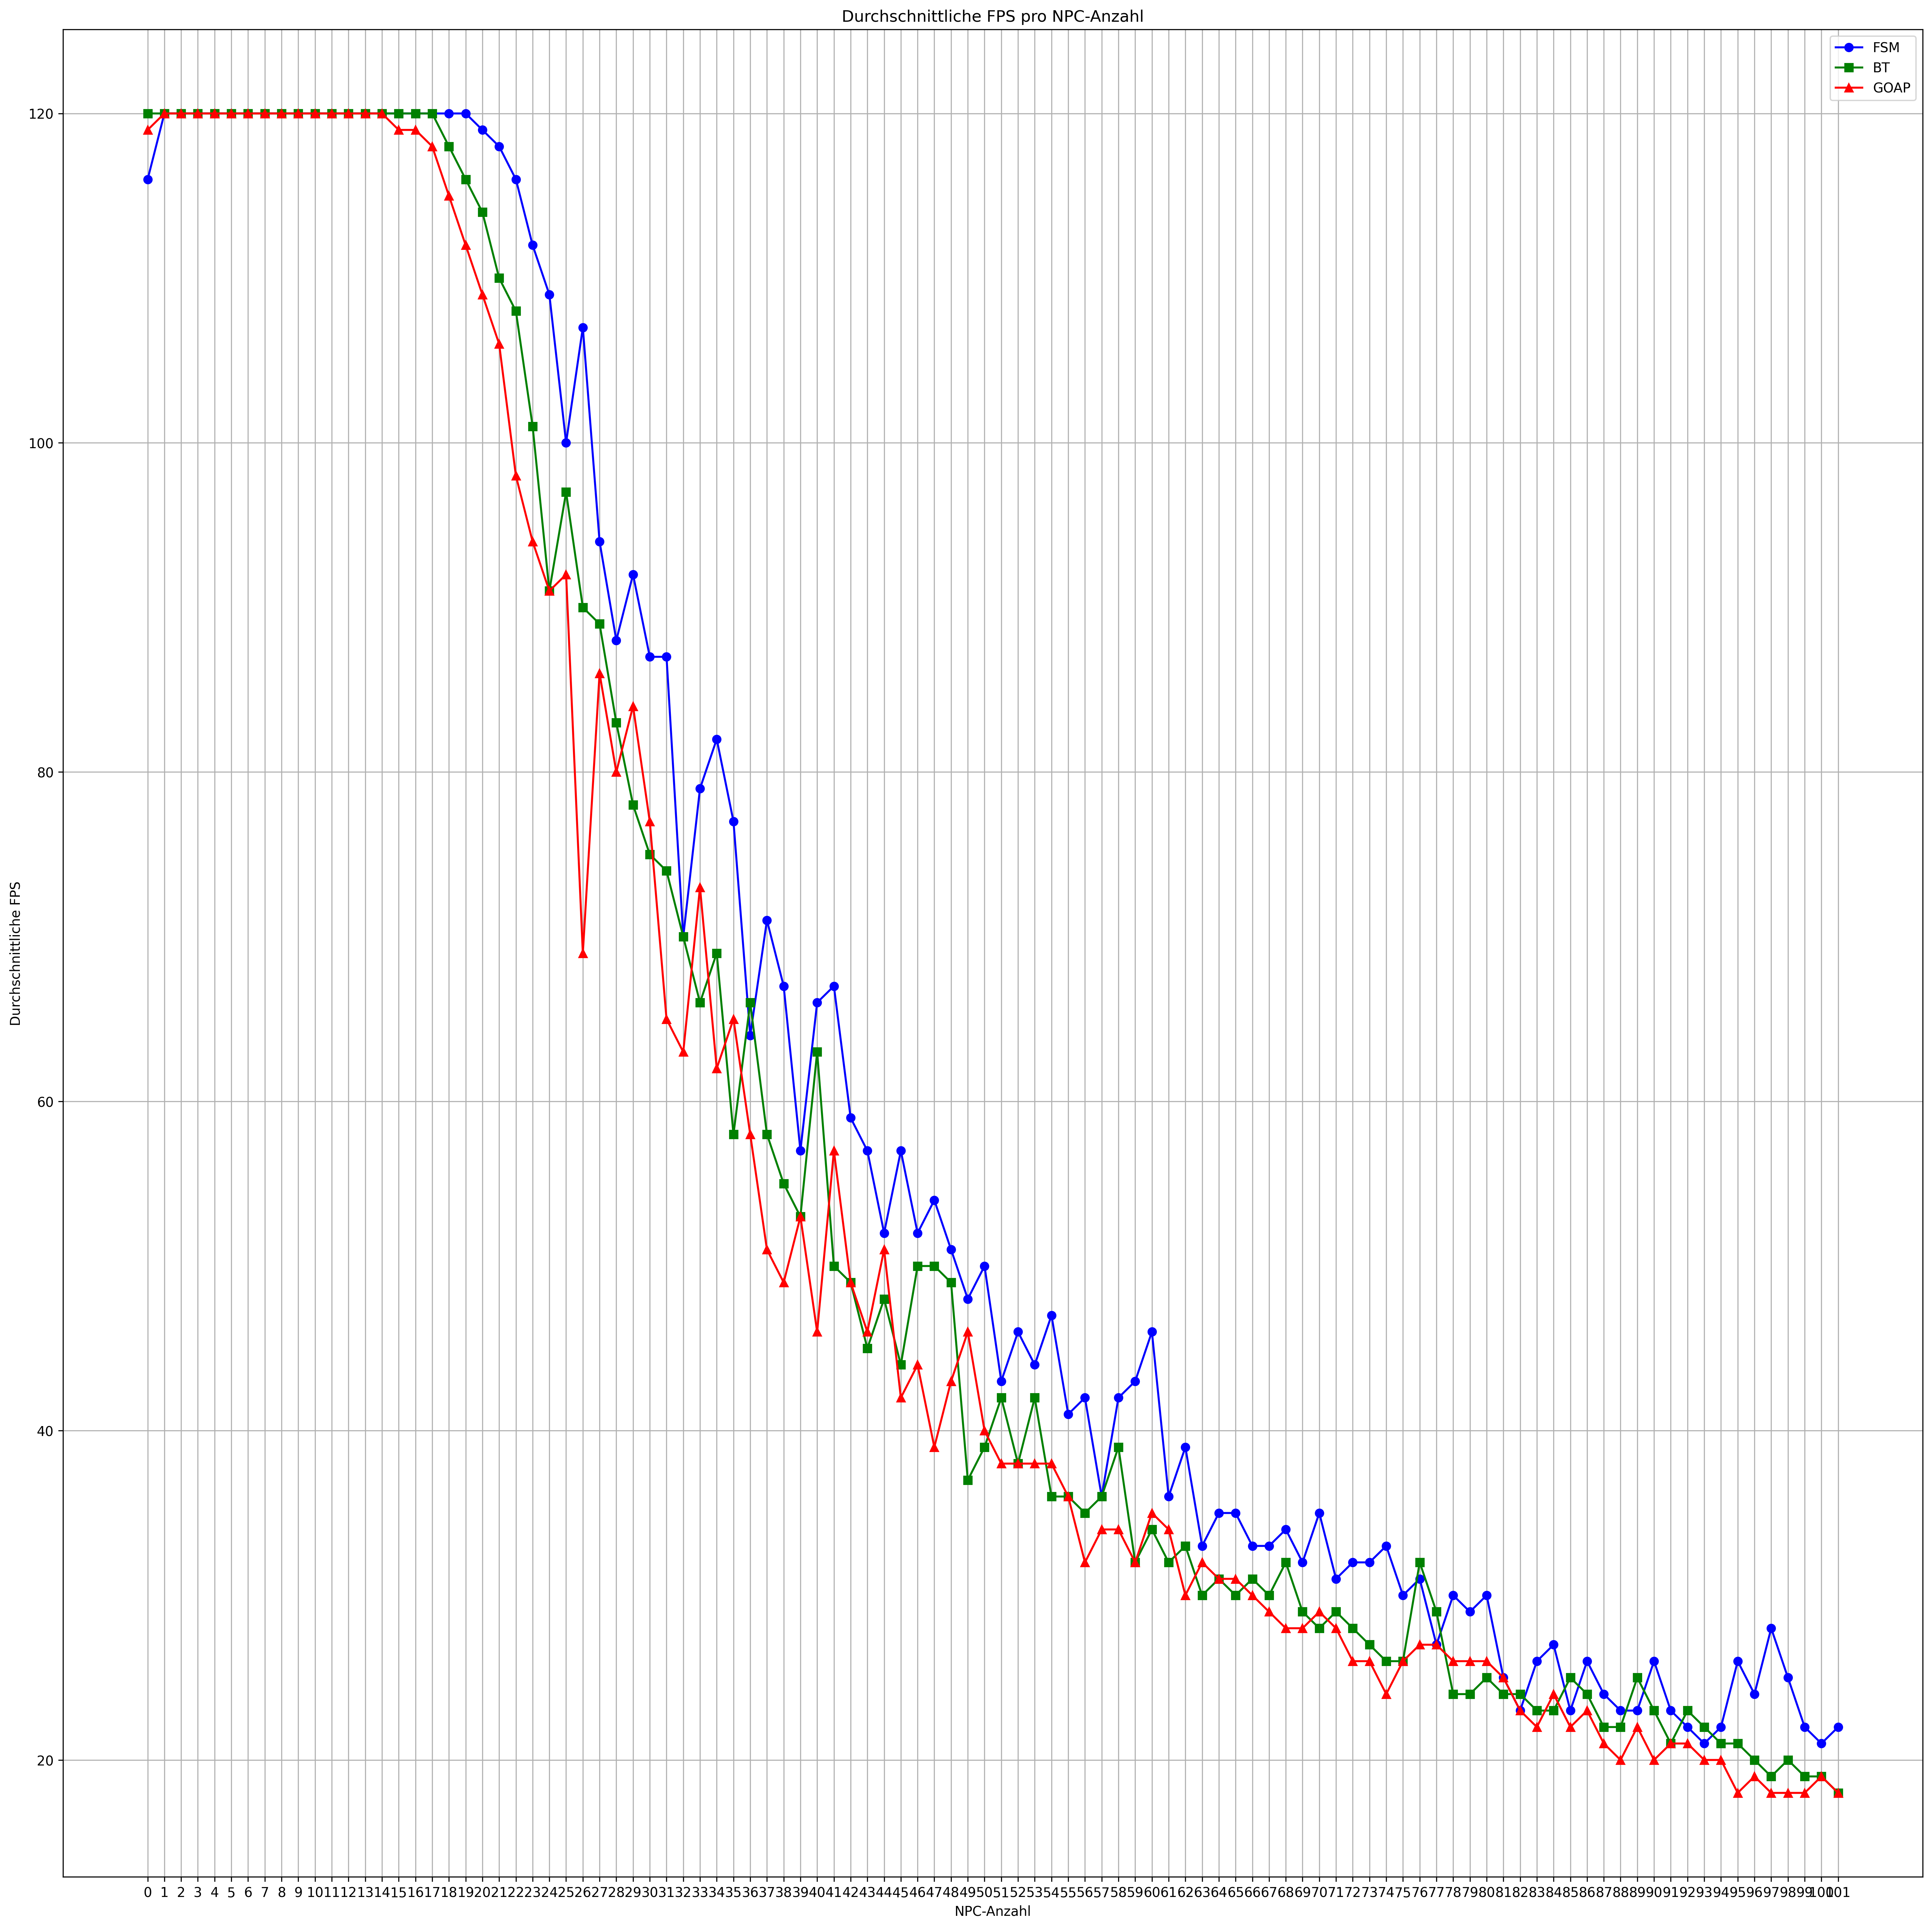
\includegraphics[width=16cm]{Vergleich/avg_fps}
	\captionsetup{justification=justified, format=plain}
  \caption{FPS-Performance Benchmark}
  \label{FPS-Performance Benchmark}
\end{figure}
